%!TeX root=../tese.tex
%("dica" para o editor de texto: este arquivo é parte de um documento maior)
% para saber mais: https://tex.stackexchange.com/q/78101


\chapter{Avaliação do MVP} \label{evaluation}

A avaliação do MVP, através do formulário de usabilidade e da atividade de aprendizado, foi realizada em sala de aula com os usuários finais. Para isso, realizamos uma atividade com a duração de uma aula de 50 minutos com uma turma de 26 alunos, entre 13 e 14 anos, do 8° ano do Ensino Fundamental II da Escola de Aplicação da Faculdade de Educação da USP (FEUSP). Durante a aula, contamos com o apoio do professor Henri Silva, que leciona matemática para a turma. 

A atividade realizada em aula foi dividade em três partes: na primeira, apresentamos um exemplo de pseudocódigo e código em Python de um programa que, dados cinco números de entrada, calcula a quantidade de números pares e de números ímpares; na segunda parte, os alunos exploraram o MVP com a simulação de forma livre; e na terceira, eles preencheram dois formulários, o de usabilidade e o da atividade de aprendizado, nessa ordem.

As 10 afirmações adaptadas do SUS e traduzidas para o português, apresentadas no formulário de usabilidade, estão enumeradas a seguir e a escala visual de Likert utilizada pode ser observada na Figura \ref{figure:likert_forms}.

\begin{enumerate}
    \item Eu gostaria de explorar mais a simulação.
    \item Eu fiquei confuso(a) muitas vezes enquanto explorava a simulação.
    \item Eu achei que a simulação foi fácil de usar.
    \item Eu precisaria de ajuda para conseguir explorar a simulação.
    \item Eu sabia o que era preciso fazer quando explorei a simulação.
    \item Algumas coisas que eu tive que fazer enquanto explorava a simulação não fizeram sentido.
    \item Eu acho que a maioria dos meus amigos podem aprender a usar a simulação muito rápido.
    \item Algumas das coisas que eu tive que fazer para explorar a simulação foram estranhas.
    \item Eu me senti confiante enquanto explorava a simulação.
    \item Eu tive que aprender muitas coisas antes de explorar a simulação.
\end{enumerate}

\begin{figure}[h!]
    \centering
    \setlength{\fboxrule}{0.1pt} % espessura da borda da figura
    \fbox{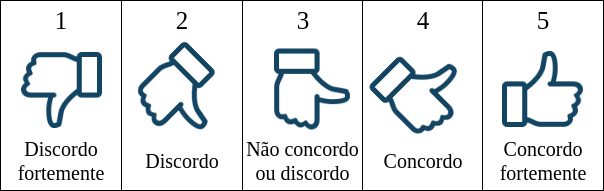
\includegraphics[scale=0.5]{escalaLikertformulario.png}}
    \caption{Representação visual da escala de Likert utilizada no formulário de usabilidade.}
    \label{figure:likert_forms}
\end{figure}

Ainda, ao final do formulário foram feitas duas perguntas dissertativas sobre o que o usuário mais gostou na simulação e o que menos gostou, além de um espaço adicional para deixar quaisquer comentários ou sugestões sobre ela.

Em relação à atividade de aprendizado, ela foi dividida em duas partes com 6 perguntas cada. Em cada pergunta, era apresentado um trecho do pseudocódigo com um ou mais conceitos de lógica de programação e era pedido para selecionar a opção que melhor representasse aquele pedaço de pseudocódigo, entre as seguintes opções: variáveis, entrada, saída, operadores, condicional e laço de repetição. A primeira parte da atividade continha perguntas sobre o pseudocódigo da simulação \enquote{Planejando a Festa}, explorada pelos estudantes. A Figura \ref{figure:atividade_festa} mostra os trechos de pseudocódigo apresentados em cada questão. A segunda parte era referente à simulação \enquote{Guardando os Brinquedos}, a qual foi apresentada no formulário, para fornecer contexto para as questões, por meio de uma imagem (Figura \ref{figure:brinquedos_forms}). Esse protótipo foi modificado do projeto dos artefatos, apresentado no Capítulo \ref{prototypes}. A figura \ref{figure:atividade_brinquedos} mostra os pedaços de pseudocódigo utilizados nessas questões.

\begin{figure}[h!]
    \centering
    \begin{subfigure}[t]{0.5\textwidth}
        \centering
        \setlength{\fboxrule}{0.1pt} % espessura da borda da figura
        \fbox{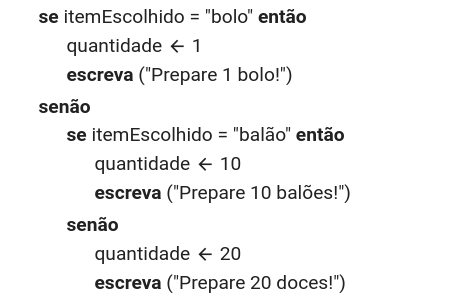
\includegraphics[scale=0.5]{figuras/atividade_festa_1.png}}
        \caption{Pseudocódigo referente à Pergunta 1}
        \label{figure:atividade_festa_1}
    \end{subfigure}
    \par\bigskip % force a bit of vertical whitespace
    \begin{subfigure}[t]{0.5\textwidth}
        \centering
        \setlength{\fboxrule}{0.1pt} % espessura da borda da figura
        \fbox{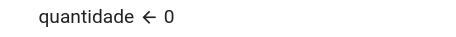
\includegraphics[scale=0.5]{figuras/atividade_festa_2.png}}
        \caption{Pseudocódigo referente à Pergunta 2}
        \label{figure:atividade_festa_2}
    \end{subfigure}
    \par\bigskip % force a bit of vertical whitespace
    \begin{subfigure}[t]{0.5\textwidth}
        \centering
        \setlength{\fboxrule}{0.1pt} % espessura da borda da figura
        \fbox{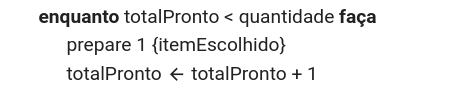
\includegraphics[scale=0.5]{figuras/atividade_festa_3.png}}
        \caption{Pseudocódigo referente à Pergunta 3}
        \label{figure:atividade_festa_3}
    \end{subfigure}
    \par\bigskip % force a bit of vertical whitespace
    \begin{subfigure}[t]{0.5\textwidth}
        \centering
        \setlength{\fboxrule}{0.1pt} % espessura da borda da figura
        \fbox{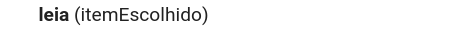
\includegraphics[scale=0.5]{figuras/atividade_festa_4.png}}
        \caption{Pseudocódigo referente à Pergunta 4}
        \label{figure:atividade_festa_4}
    \end{subfigure}
    \par\bigskip % force a bit of vertical whitespace
    \begin{subfigure}[t]{0.5\textwidth}
        \centering
        \setlength{\fboxrule}{0.1pt} % espessura da borda da figura
        \fbox{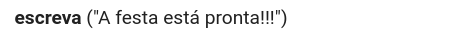
\includegraphics[scale=0.5]{figuras/atividade_festa_5.png}}
        \caption{Pseudocódigo referente à Pergunta 5}
        \label{figure:atividade_festa_5}
    \end{subfigure}
    \par\bigskip % force a bit of vertical whitespace
    \begin{subfigure}[t]{0.5\textwidth}
        \centering
        \setlength{\fboxrule}{0.1pt} % espessura da borda da figura
        \fbox{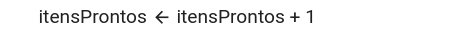
\includegraphics[scale=0.5]{figuras/atividade_festa_6.png}}
        \caption{Pseudocódigo referente à Pergunta 6}
        \label{figure:atividade_festa_6}
    \end{subfigure}
    \caption{Trechos de pseudocódigo apresentados em cada pergunta da atividade de aprendizado referente à simulação \enquote{Planejando a Festa}.}
    \label{figure:atividade_festa}
\end{figure}

\begin{figure}[h!]
    \centering
    \setlength{\fboxrule}{0.1pt} % espessura da borda da figura
    \fbox{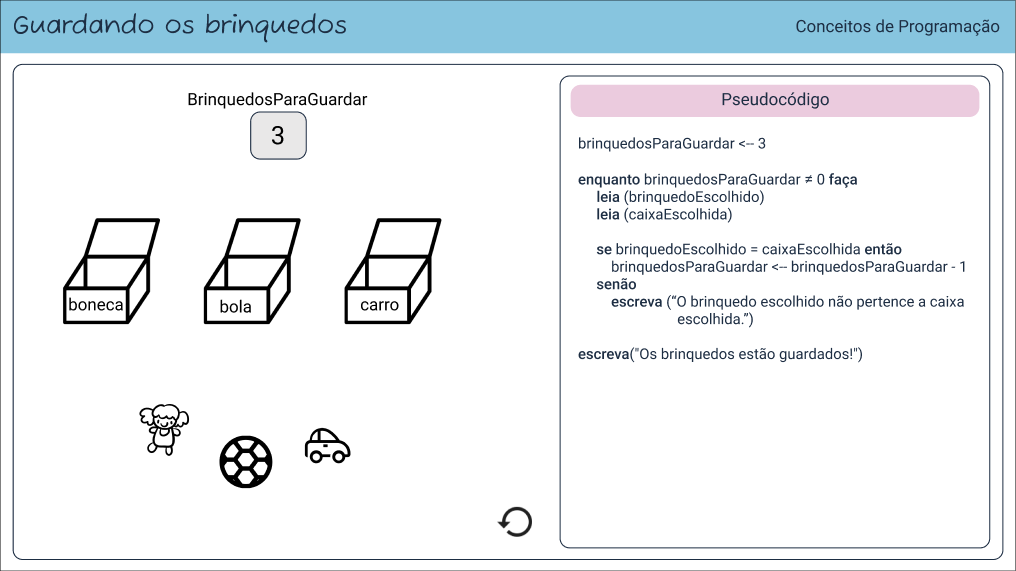
\includegraphics[scale=0.45]{prototipo_brinquedos_formulario.png}}
    \caption{Protótipo da simulação \enquote{Guardando os Brinquedos} apresentado na atividade de aprendizado para fornecer contexto para as questões.}
    \label{figure:brinquedos_forms}
\end{figure}

\begin{figure}[h!]
    \centering
    \begin{subfigure}[t]{0.5\textwidth}
        \centering
        \setlength{\fboxrule}{0.1pt} % espessura da borda da figura
        \fbox{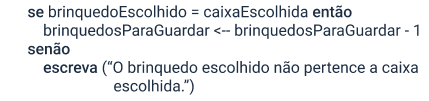
\includegraphics[scale=0.5]{figuras/atividade_brinquedos_1.png}}
        \caption{Pseudocódigo referente à Pergunta 1}
        \label{figure:atividade_brinquedos_1}
    \end{subfigure}
    \par\bigskip % force a bit of vertical whitespace
    \begin{subfigure}[t]{0.5\textwidth}
        \centering
        \setlength{\fboxrule}{0.1pt} % espessura da borda da figura
        \fbox{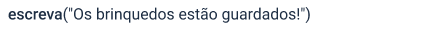
\includegraphics[scale=0.5]{figuras/atividade_brinquedos_2.png}}
        \caption{Pseudocódigo referente à Pergunta 2}
        \label{figure:atividade_brinquedos_2}
    \end{subfigure}
    \par\bigskip % force a bit of vertical whitespace
    \begin{subfigure}[t]{0.5\textwidth}
        \centering
        \setlength{\fboxrule}{0.1pt} % espessura da borda da figura
        \fbox{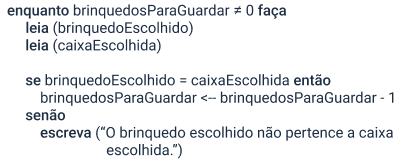
\includegraphics[scale=0.5]{figuras/atividade_brinquedos_3.png}}
        \caption{Pseudocódigo referente à Pergunta 3}
        \label{figure:atividade_brinquedos_3}
    \end{subfigure}
    \par\bigskip % force a bit of vertical whitespace
    \begin{subfigure}[t]{0.5\textwidth}
        \centering
        \setlength{\fboxrule}{0.1pt} % espessura da borda da figura
        \fbox{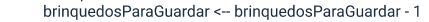
\includegraphics[scale=0.5]{figuras/atividade_brinquedos_4.png}}
        \caption{Pseudocódigo referente à Pergunta 4}
        \label{figure:atividade_brinquedos_4}
    \end{subfigure}
    \par\bigskip % force a bit of vertical whitespace
    \begin{subfigure}[t]{0.5\textwidth}
        \centering
        \setlength{\fboxrule}{0.1pt} % espessura da borda da figura
        \fbox{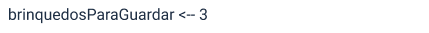
\includegraphics[scale=0.5]{figuras/atividade_brinquedos_5.png}}
        \caption{Pseudocódigo referente à Pergunta 5}
        \label{figure:atividade_brinquedos_5}
    \end{subfigure}
    \par\bigskip % force a bit of vertical whitespace
    \begin{subfigure}[t]{0.5\textwidth}
        \centering
        \setlength{\fboxrule}{0.1pt} % espessura da borda da figura
        \fbox{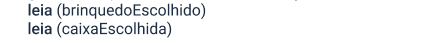
\includegraphics[scale=0.5]{figuras/atividade_brinquedos_6.png}}
        \caption{Pseudocódigo referente à Pergunta 6}
        \label{figure:atividade_brinquedos_6}
    \end{subfigure}
    \caption{Trechos de pseudocódigo apresentados em cada pergunta da atividade de aprendizado referente à simulação \enquote{Guardando os Brinquedos}.}
    \label{figure:atividade_brinquedos}
\end{figure}

O Capítulo a seguir apresenta os resultados da avaliação do MVP feita a partir das respostas dos formulários.
